\documentclass[12pt, notitlepage, final]{article} 

\newcommand{\name}{Vince Coghlan}

\usepackage{amsfonts}
\usepackage{amssymb}
\usepackage{amsmath}
\usepackage{latexsym}
\usepackage{enumerate}
\usepackage{amsthm}
\usepackage{nccmath}
\usepackage{setspace}
\usepackage[pdftex]{graphicx}
\usepackage{epstopdf}
\usepackage[siunitx]{circuitikz}
\usepackage{tikz}
\usepackage{float}
\usepackage{cancel} 
\usepackage{setspace}
\usepackage{overpic}
\usepackage{mathtools}
\usepackage{listings}
\usepackage{color}

\numberwithin{equation}{section}
\DeclareRobustCommand{\beginProtected}[1]{\begin{#1}}
\DeclareRobustCommand{\endProtected}[1]{\end{#1}}
\newcommand{\dbr}[1]{d_{\mbox{#1BR}}}
\newtheorem{lemma}{Lemma}
\newtheorem*{corollary}{Corollary}
\newtheorem{theorem}{Theorem}
\newtheorem{proposition}{Proposition}
\theoremstyle{definition}
\newtheorem{define}{Definition}
\newcommand{\column}[2]{
\left( \begin{array}{ccc}
#1 \\
#2
\end{array} \right)}

\newdimen\digitwidth
\settowidth\digitwidth{0}
\def~{\hspace{\digitwidth}}

\setlength{\parskip}{1pc}
\setlength{\parindent}{0pt}
\setlength{\topmargin}{-3pc}
\setlength{\textheight}{9.0in}
\setlength{\oddsidemargin}{0pc}
\setlength{\evensidemargin}{0pc}
\setlength{\textwidth}{6.5in}
\newcommand{\answer}[1]{\newpage\noindent\framebox{\vbox{{\bf ECEN 3400 Spring 2014} 
\hfill {\bf \name} \vspace{-1cm}
\begin{center}{Homework \#3}\end{center} } }\bigskip }

%absolute value code
\DeclarePairedDelimiter\abs{\lvert}{\rvert}%
\DeclarePairedDelimiter\norm{\lVert}{\rVert}
\makeatletter
\let\oldabs\abs
\def\abs{\@ifstar{\oldabs}{\oldabs*}}
%
\let\oldnorm\norm
\def\norm{\@ifstar{\oldnorm}{\oldnorm*}}
\makeatother

\def\dbar{{\mathchar'26\mkern-12mu d}}
\def \Frac{\displaystyle\frac}
\def \Sum{\displaystyle\sum}
\def \Int{\displaystyle\int}
\def \Prod{\displaystyle\prod}
\def \P[x]{\Frac{\partial}{\partial x}}
\def \D[x]{\Frac{d}{dx}}
\newcommand{\PD}[2]{\frac{\partial#1}{\partial#2}}
\newcommand{\PF}[1]{\frac{\partial}{\partial#1}}
\newcommand{\DD}[2]{\frac{d#1}{d#2}}
\newcommand{\DF}[1]{\frac{d}{d#1}}
\newcommand{\fix}[2]{\left(#1\right)_#2}
\newcommand{\ket}[1]{|#1\rangle}
\newcommand{\bra}[1]{\langle#1|}
\newcommand{\braket}[2]{\langle #1 | #2 \rangle}
\newcommand{\bopk}[3]{\langle #1 | #2 | #3 \rangle}
\newcommand{\Choose}[2]{\displaystyle {#1 \choose #2}}
\newcommand{\proj}[1]{\ket{#1}\bra{#1}}
\def\del{\vec{\nabla}}
\newcommand{\avg}[1]{\langle#1\rangle}
\newcommand{\piecewise}[4]{\left\{\beginProtected{array}{rl}#1&:#2\\#3&:#4\endProtected{array}\right.}
\newcommand{\systeme}[2]{\left\{\beginProtected{array}{rl}#1\\#2\endProtected{array}\right.}
\def \KE{K\!E}
\def\Godel{G$\ddot{\mbox{o}}$del}

\onehalfspacing

\begin{document}

\answer{}
1) \textbf{9.18:}
\begin{figure}[H]
\begin{center}
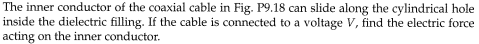
\includegraphics[width=14cm]{p1a}
\end{center}
\end{figure}
\begin{figure}[H]
\begin{center}
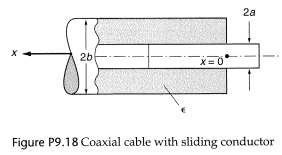
\includegraphics[width=8cm]{p1b}
\end{center}
\end{figure}

The capacitance of a length of cable will be:
\[
  C = \frac{2\pi \epsilon_1 x}{\ln(b/a)} + \frac{2\pi \epsilon_0(L-x)}{\ln(b/a)}
\]

The Electric force will be:
\[
  F = \frac{dW}{dx}
\]
where
\[
  W = \frac{1}{2}CV^2 = \frac{1}{2}(\frac{2\pi \epsilon_1 x}{\ln(b/a)} + \frac{2\pi \epsilon_0(L-x)}{\ln(b/a)})V^2
\]
This means that:
\[
  F = \frac{V^2 \pi (\epsilon_1 - \epsilon_0)}{\ln(b/a)}
\]

\newpage

2) \textbf{10.3:}
\begin{figure}[H]
\begin{center}
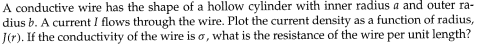
\includegraphics[width=14cm]{p2}
\end{center}
\end{figure}

The current density will be
\[
  J = \frac{I}{A} = \frac{I}{\pi b^2 - \pi a^2}
\]
The resistance of the wire will be $\frac{A}{\sigma L}$ and so the resistance per unit length
will be $\frac{A}{\sigma}$ or $\frac{\pi(b^2 - a^2)}{\sigma}$.

3) \textbf{10.8:}
\begin{figure}[H]
\begin{center}
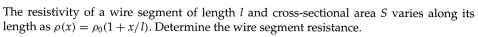
\includegraphics[width=14cm]{p3}
\end{center}
\end{figure}
Since
\[
  \rho(x) = \rho_0(1+x/l)
\]
and
\[
  R = \rho\frac{l}{A}
\]
then
\[
  R(x) = \rho_0(1 + \frac{x}{l})\frac{l}{A}
\]
\[
  R(x) = \frac{\rho_0 l}{A} + \frac{\rho_0 x}{A}
\]

\newpage

4) \textbf{11.11:}
\begin{figure}[H]
\begin{center}
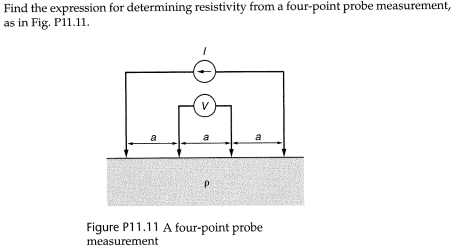
\includegraphics[width=14cm]{p4}
\end{center}
\end{figure}

The potential we are going to measure can be found as in the example problem:
\[
  V = \int_{\text{probe 1}}^{\text{probe 2}} E \cdot dl = \int_{\text{probe 1}}^{\text{probe 2}} \rho J \cdot dl
\]
The first thing we need to do is find the current density:
\[
  J = \frac{I}{A}
\]
Then we can form the integral:
\[
  V = \int_{\text{probe 1}}^{\text{probe 2}} \frac{RI}{l} \cdot dl = RI\ln{2a}
\]
And we find
\[
  \rho = \frac{Vl}{IA\ln{2a}}
\]
According to the internet the equation should be:
\[
  \rho = \frac{V\pi}{I\ln{2}}
\]
Which is not what I have, so I dont know where I went wrong.
\newpage
5) \textbf{12.6:}
\begin{figure}[H]
\begin{center}
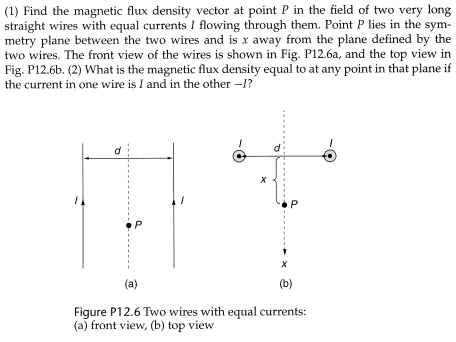
\includegraphics[width=14cm]{p5}
\end{center}
\end{figure}
6) \textbf{12.7:}
\begin{figure}[H]
\begin{center}
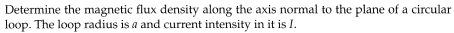
\includegraphics[width=14cm]{p6}
\end{center}
\end{figure}
7)
\begin{figure}[H]
\begin{center}
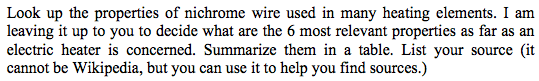
\includegraphics[width=14cm]{p7}
\end{center}
\end{figure}
8)
\begin{figure}[H]
\begin{center}
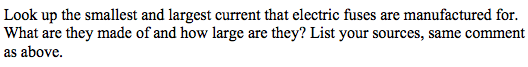
\includegraphics[width=14cm]{p8}
\end{center}
\end{figure}



\end{document}
